\usepackage{graphicx}
\thispagestyle{fancy}
\vspace*{\fill}
\subsection{Tela de comandos da máquina}
Para acessar esta tela da inicial basta clicar em comandos no menu inferior. Ao iniciar a máquina com exceção da tela de ajuda, alarmes e velocidade; esta é a única tela é possível acessar com a máquina desabilitada. Ao habilitar a máquina o menu de ajustes, pedido, configuração, a tela de comandos das outras unidades e próxima página de comandos de máquina ficam disponíveis.

O menu superior esquerdo leva a tela de comandos de cada uma das unidades, o botão "\textgreater" no menu superior esquerdo leva a tela de comandos da alimentação, o botão "\textgreater" no canto direito leva a segunda tela de comandos de máquina e o "ajustes" como não existe uma tela de ajuste de máquina leva a tela de ajustes da alimentação.
\vspace*{10pt}

\begin{figure}
    \centering
    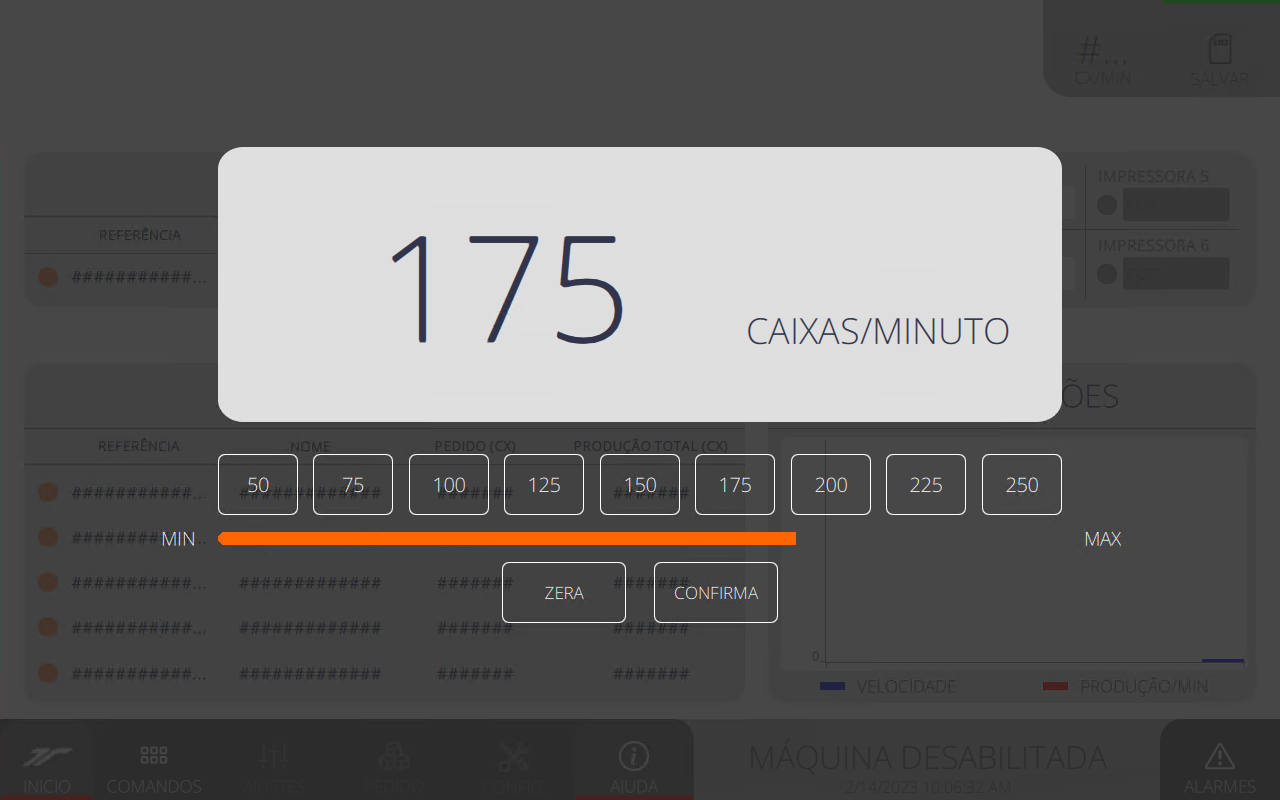
\includegraphics[width=480,height=300]{imagesICV/02-machine/1}
    \caption{Tela principal}
    \label{fig:}
\end{figure}
\newpage
\thispagestyle{fancy}
\vspace{\fill}

\subsection{Velocidade da máquina}
\begin{figure}
    \centering
    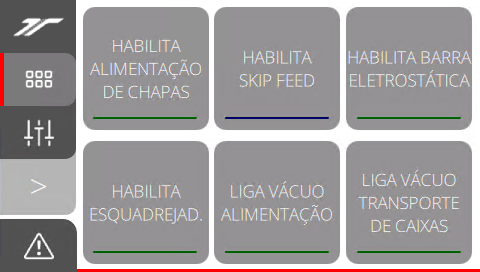
\includegraphics[width=576,height=360]{imagesICV/02-machine/2}
    \caption{Velocidade da máquina}
    \label{fig:}
\end{figure}
\newpage
\thispagestyle{fancy}
\vspace{\fill}

\subsection{Acionamento da máquina}
\begin{figure}
    \centering
    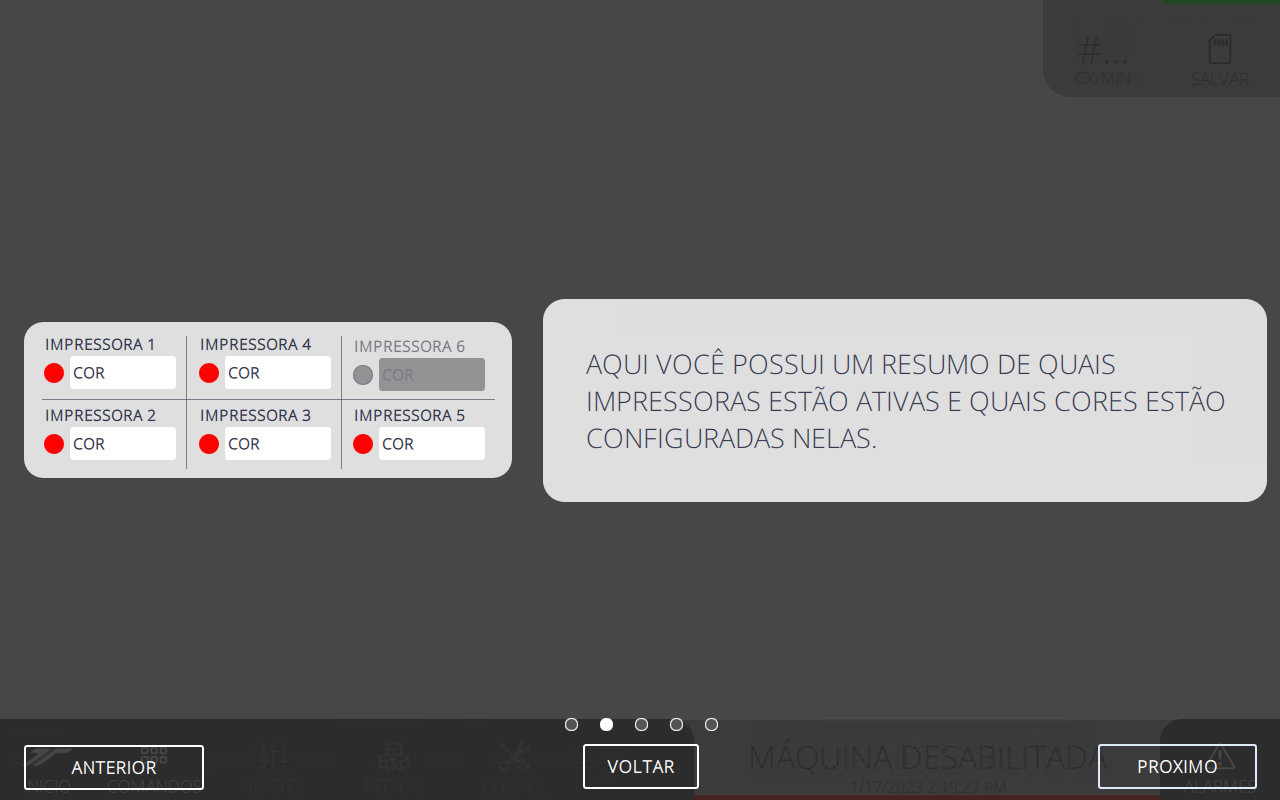
\includegraphics[width=576,height=360]{imagesICV/02-machine/3}
    \caption{Acionamento da máquina}
    \label{fig:}
\end{figure}
\newpage
\thispagestyle{fancy}
\vspace{\fill}

\subsection{Executa ponto zero geral}
\begin{figure}
    \centering
    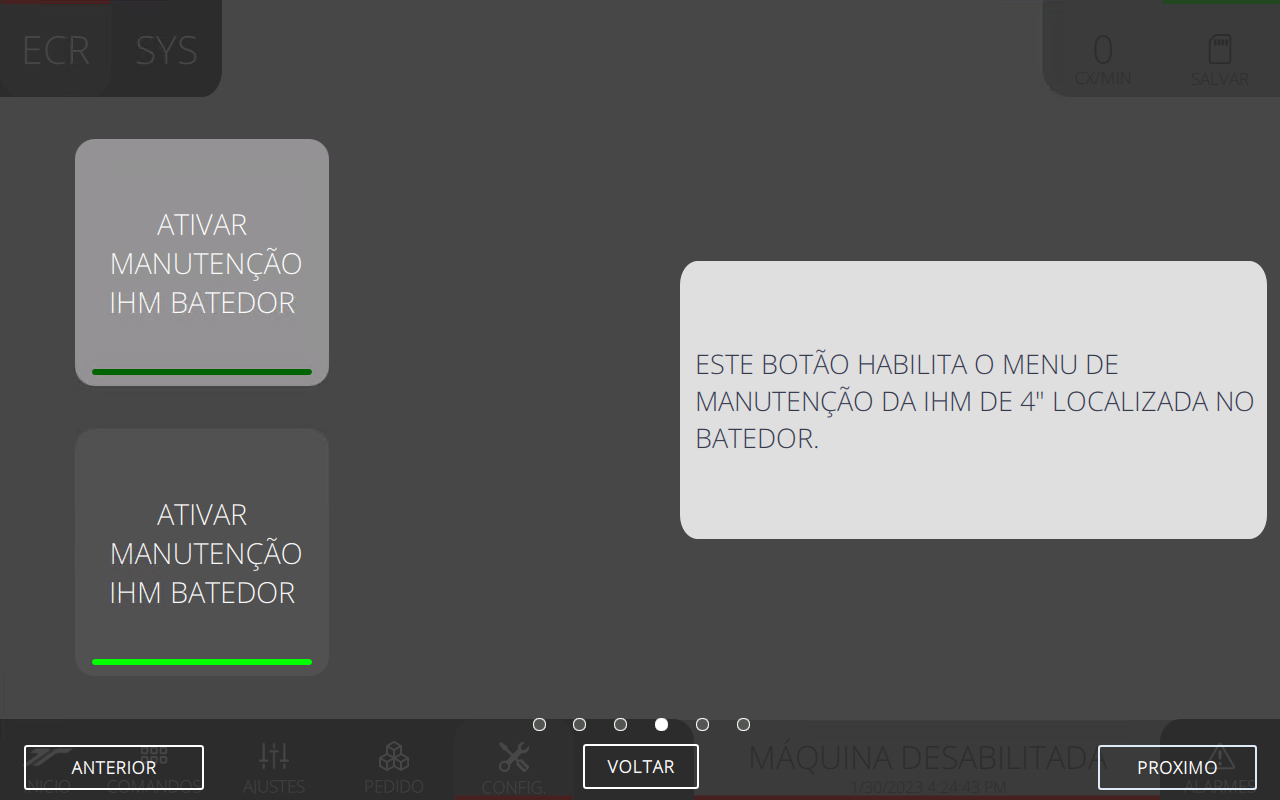
\includegraphics[width=576,height=360]{imagesICV/02-machine/4}
    \caption{Executa ponto zero da máquina}
    \label{fig:}
\end{figure}
\newpage
\thispagestyle{fancy}
\vspace{\fill}

\subsection{Habilita máquina}
\begin{figure}
    \centering
    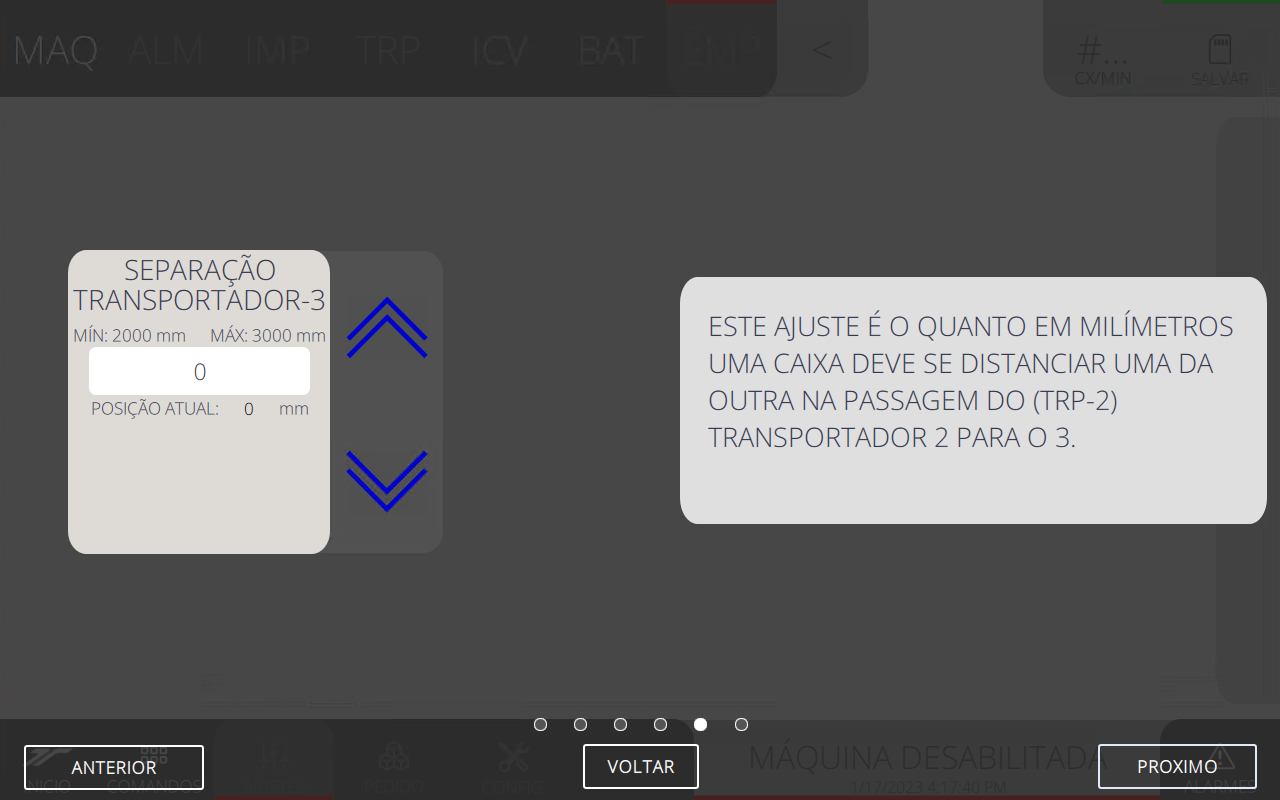
\includegraphics[width=576,height=360]{imagesICV/02-machine/5}
    \caption{Habilita máquina}
    \label{fig:}
\end{figure}
\newpage
\thispagestyle{fancy}
\vspace{\fill}

\subsection{Habilita vácuo transporte}
\begin{figure}
    \centering
    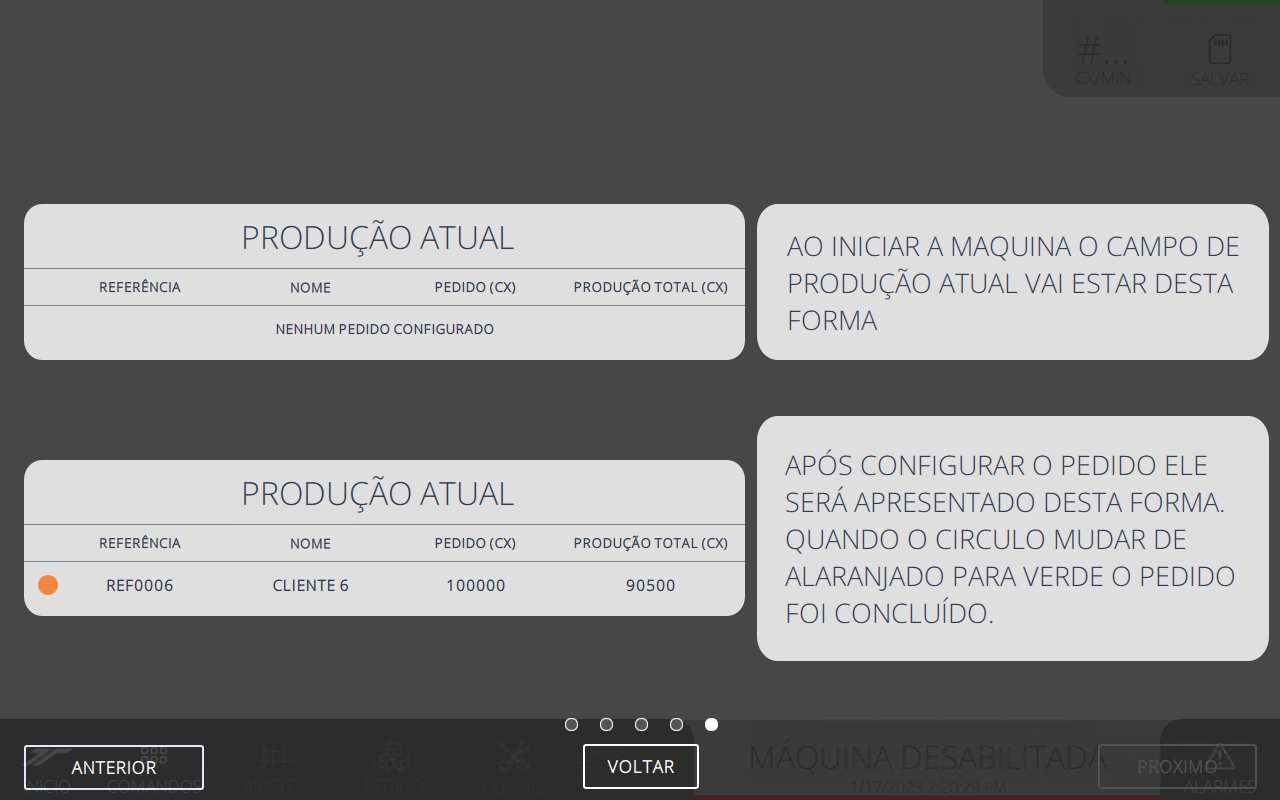
\includegraphics[width=576,height=360]{imagesICV/02-machine/6}
    \caption{Habilita vácuo transporte}
    \label{fig:}
\end{figure}
\newpage
\thispagestyle{fancy}
\vspace{\fill}

\subsection{Habilita skip feed}
\begin{figure}
    \centering
    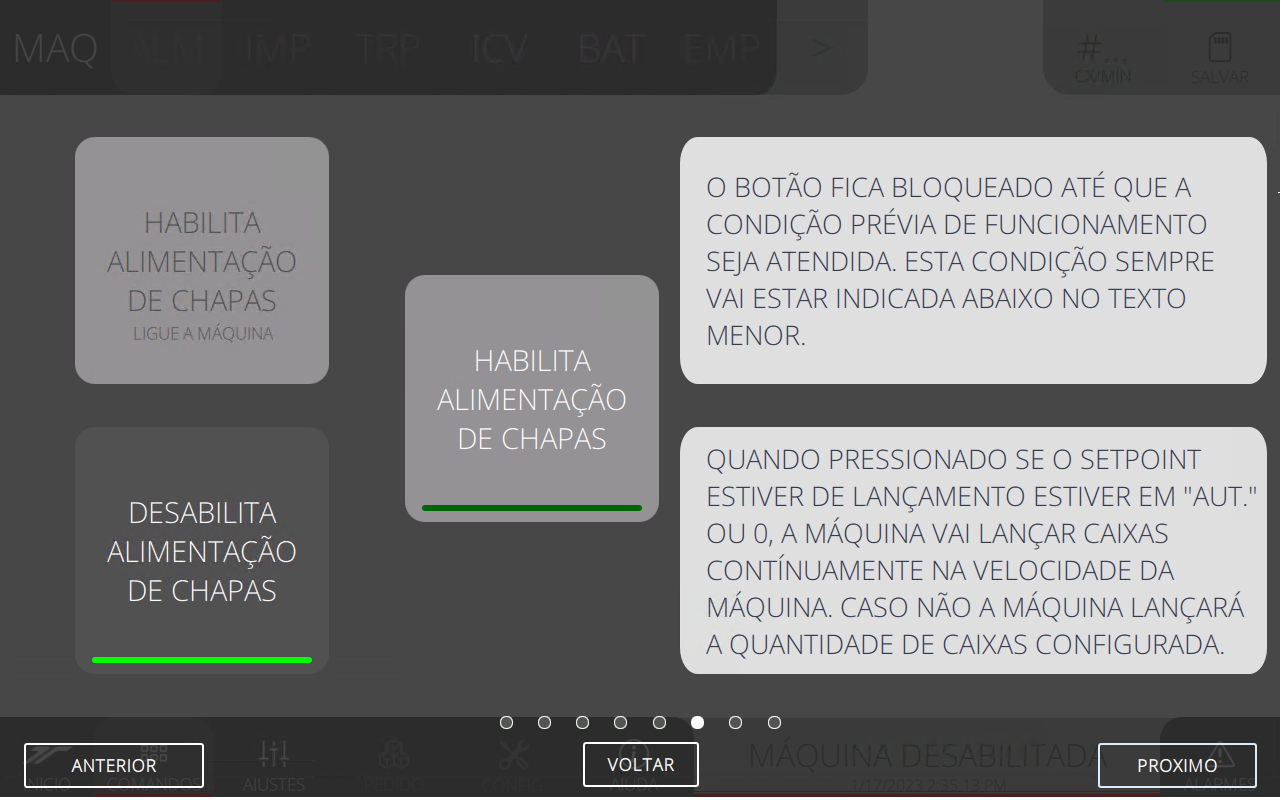
\includegraphics[width=576,height=360]{imagesICV/02-machine/7}
    \caption{Habilita skip feed}
    \label{fig:}
\end{figure}
\newpage
\thispagestyle{fancy}
\vspace{\fill}

\subsection{Liga controle do embuchamento}
\begin{figure}
    \centering
    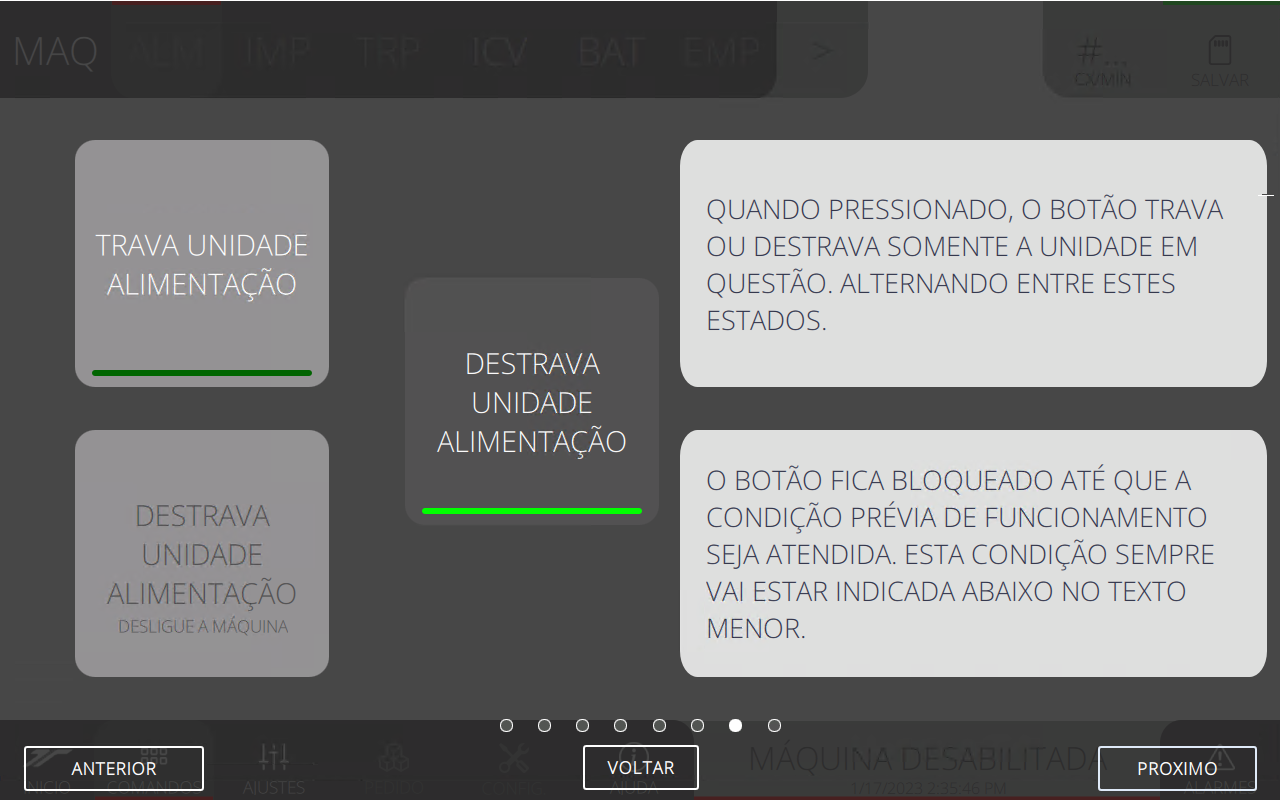
\includegraphics[width=576,height=360]{imagesICV/02-machine/8}
    \caption{Liga controle do embuchamento}
    \label{fig:}
\end{figure}

